% Native editable composition from verified, unchanged IDE images.
\par
\begin{figure}[htbp]
  \centering
  \sbox0{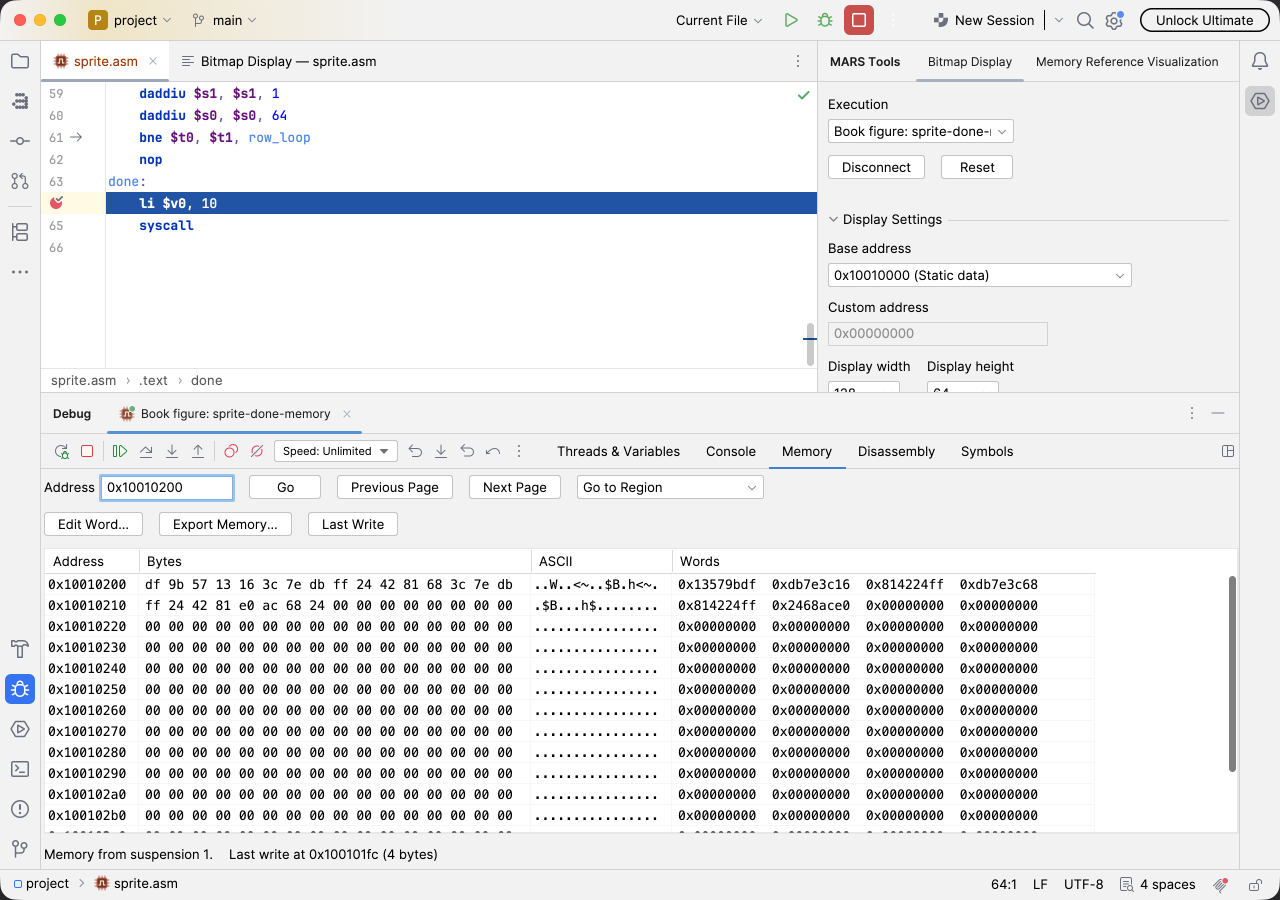
\includegraphics[artifact]{packages/003-eight-byte-sprite/captures/f04-complete-sprite/memory.png}}
  \sbox2{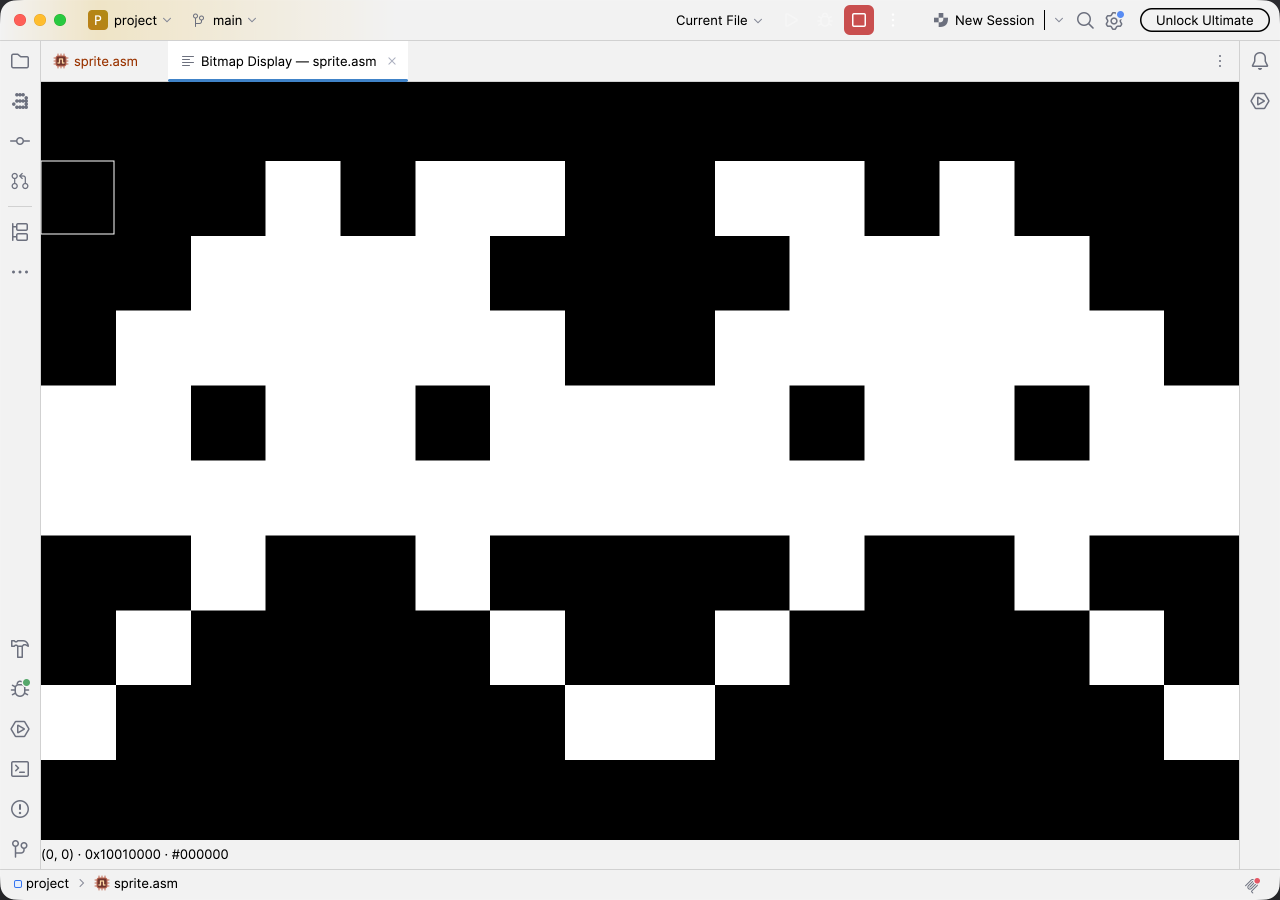
\includegraphics[artifact]{packages/003-eight-byte-sprite/captures/f04-complete-sprite/bitmap.png}}
  \edef\MARSdonesourceLeft{\the\dimexpr0.036718750\wd0\relax}
  \edef\MARSdonesourceBottom{\the\dimexpr0.757777778\ht0\relax}
  \edef\MARSdonesourceRight{\the\dimexpr0.611718750\wd0\relax}
  \edef\MARSdonesourceTop{\the\dimexpr0.188888889\ht0\relax}
  \edef\MARSdonebitmapLeft{\the\dimexpr0.032031250\wd2\relax}
  \edef\MARSdonebitmapBottom{\the\dimexpr0.155555556\ht2\relax}
  \edef\MARSdonebitmapRight{\the\dimexpr0.032031250\wd2\relax}
  \edef\MARSdonebitmapTop{\the\dimexpr0.178888889\ht2\relax}
  \edef\MARSdonememoryLeft{\the\dimexpr0.034375000\wd0\relax}
  \edef\MARSdonememoryBottom{\the\dimexpr0.311111111\ht0\relax}
  \edef\MARSdonememoryRight{\the\dimexpr0.578906250\wd0\relax}
  \edef\MARSdonememoryTop{\the\dimexpr0.608888889\ht0\relax}
  \begin{tikzpicture}[alt={Three annotated IDE details at done, before li v0 ten. The 16-column eight-row display has the original image on the left and its horizontal mirror on the right. Memory at 10010200 contains the unchanged frame canary, all eight source bytes and the first four reversed bytes. The next memory row starts with the last four reversed bytes followed by the unchanged rows canary.}]
    \node[anchor=north west,inner sep=0,font=\small\bfseries] (source-title) at (6mm,0) {All eight rows have been processed};
    \node[anchor=north west,inner sep=0] (source) at ([yshift=-1mm]source-title.south west) {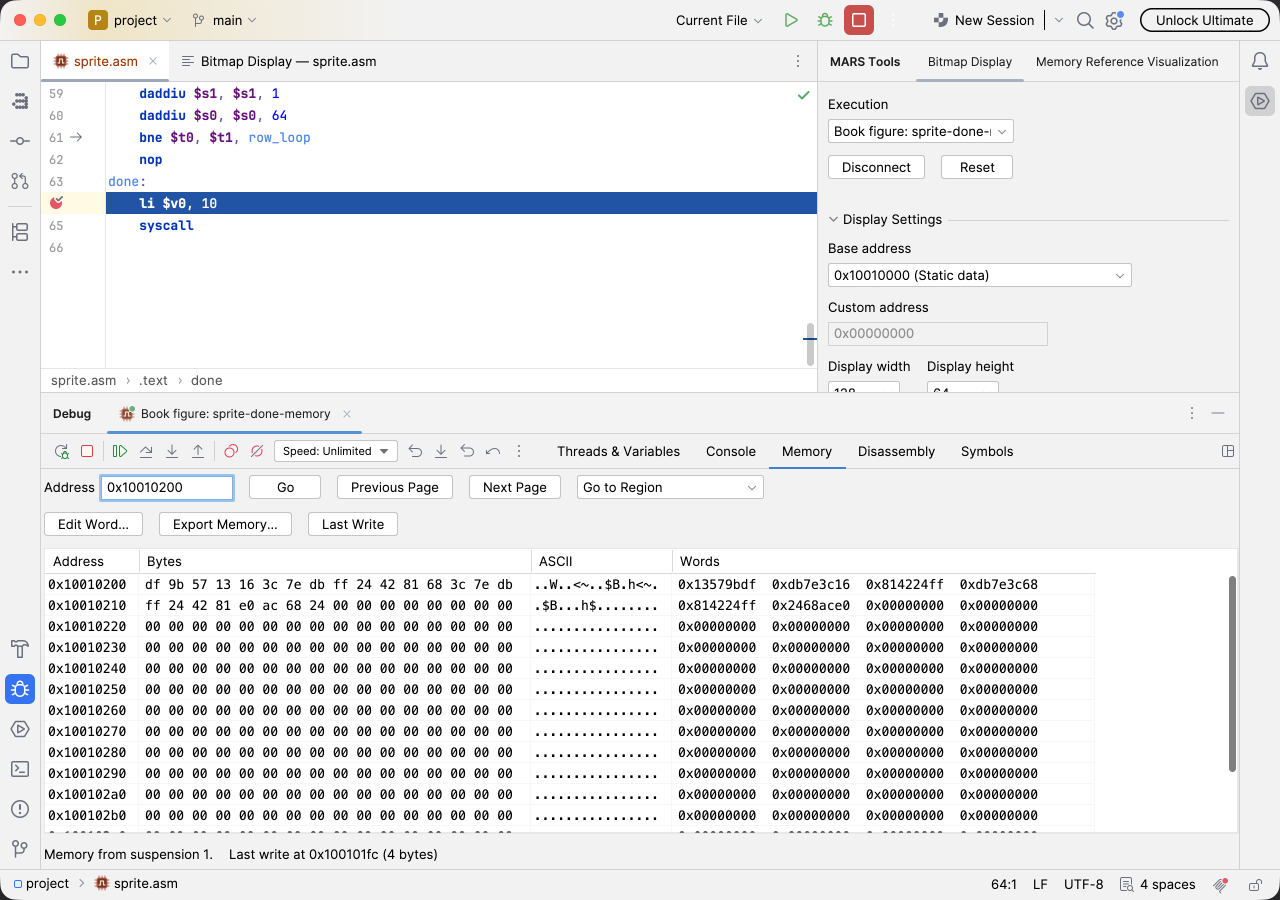
\includegraphics[width=0.7\linewidth,artifact,trim={\MARSdonesourceLeft{} \MARSdonesourceBottom{} \MARSdonesourceRight{} \MARSdonesourceTop{}},clip]{packages/003-eight-byte-sprite/captures/f04-complete-sprite/memory.png}};
    \begin{scope}[shift={(source.south west)},x={($(source.south east)-(source.south west)$)},y={($(source.north west)-(source.south west)$)}]
      \draw[black,line width=0.7pt] (0.135555556,0.083333333) rectangle (0.377777778,0.541666667);
      \node[draw=black,fill=white,circle,inner sep=1.5pt,font=\footnotesize] at ($(0.135555556,0.541666667)+(-3mm,0)$) {1};
    \end{scope}
    \node[anchor=north west,inner sep=0,font=\small\bfseries] (bitmap-title) at ([yshift=-2mm]source.south west) {Original image on the left; horizontal mirror on the right};
    \node[anchor=north west,inner sep=0] (bitmap) at ([yshift=-1mm]bitmap-title.south west) {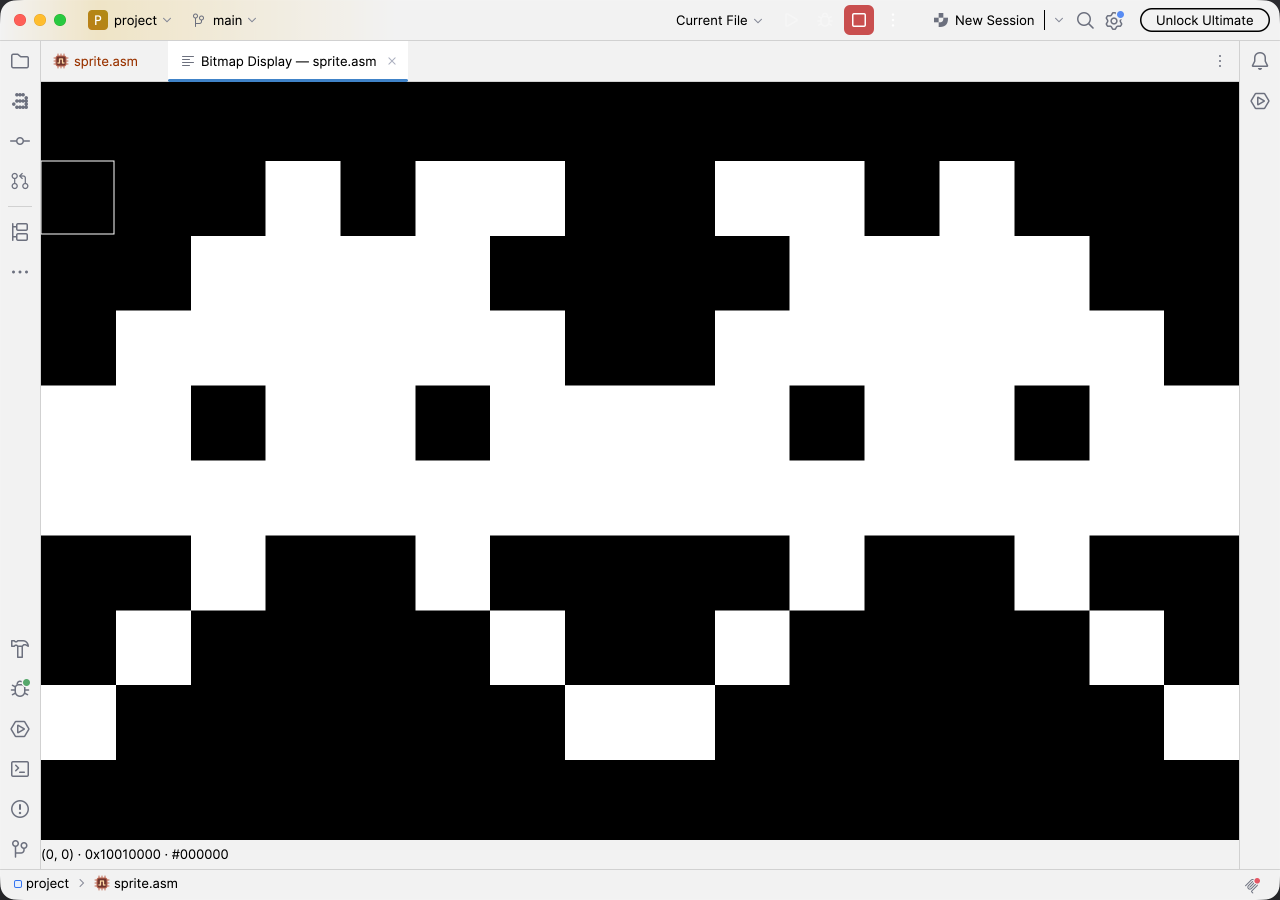
\includegraphics[width=0.84\linewidth,artifact,trim={\MARSdonebitmapLeft{} \MARSdonebitmapBottom{} \MARSdonebitmapRight{} \MARSdonebitmapTop{}},clip]{packages/003-eight-byte-sprite/captures/f04-complete-sprite/bitmap.png}};
    \begin{scope}[shift={(bitmap.south west)},x={($(bitmap.south east)-(bitmap.south west)$)},y={($(bitmap.north west)-(bitmap.south west)$)}]
      \draw[black,line width=0.7pt] (0.000000000,0.000000000) rectangle (1.000000000,1.000000000);
      \node[draw=black,fill=white,circle,inner sep=1.5pt,font=\footnotesize] at ($(0.000000000,1.000000000)+(-3mm,0)$) {2};
    \end{scope}
    \node[anchor=north west,inner sep=0,font=\small\bfseries] (memory-title) at ([yshift=-2mm]bitmap.south west) {Source, reversed bytes and both retained canaries};
    \node[anchor=north west,inner sep=0] (memory) at ([yshift=-1mm]memory-title.south west) {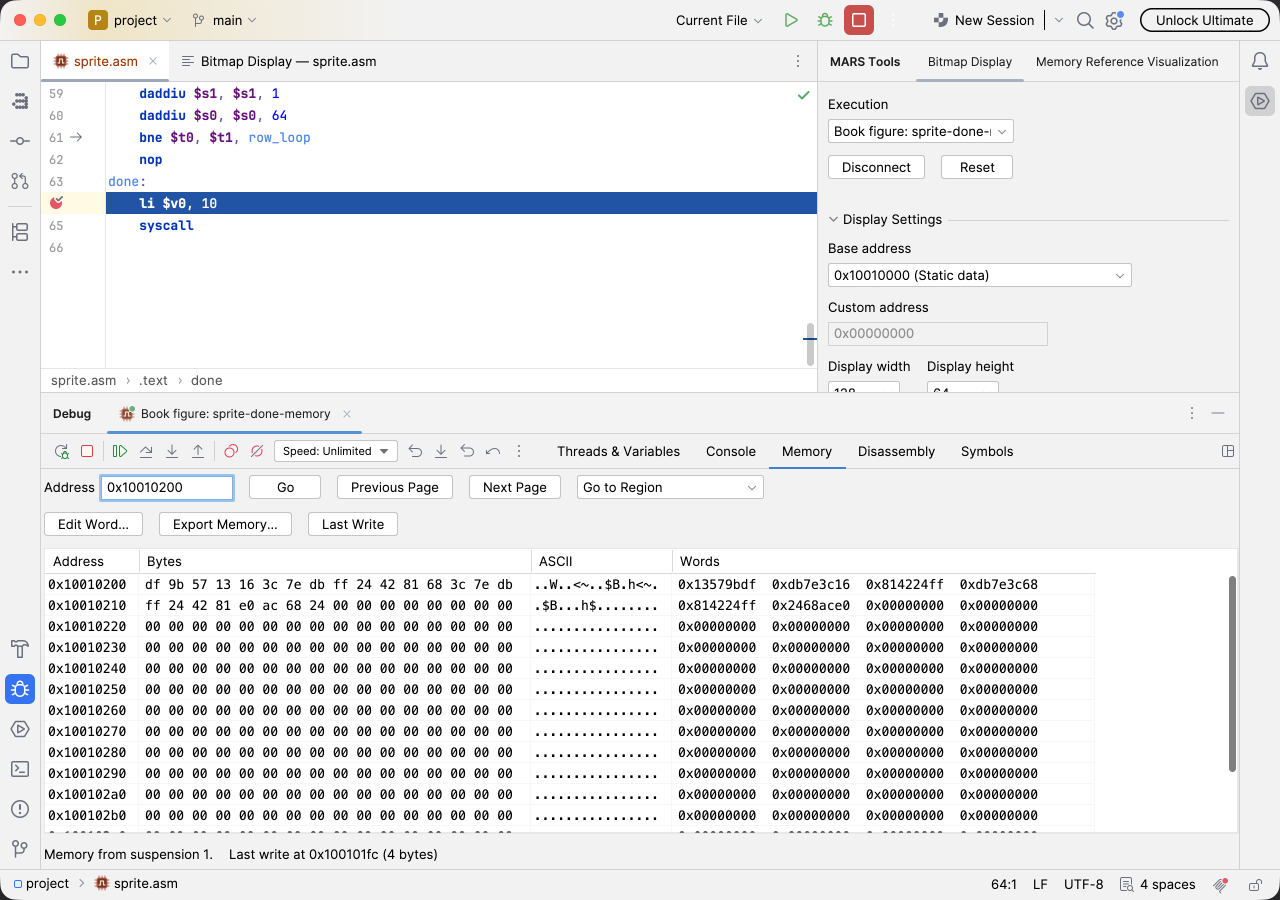
\includegraphics[width=0.84\linewidth,artifact,trim={\MARSdonememoryLeft{} \MARSdonememoryBottom{} \MARSdonememoryRight{} \MARSdonememoryTop{}},clip]{packages/003-eight-byte-sprite/captures/f04-complete-sprite/memory.png}};
    \begin{scope}[shift={(memory.south west)},x={($(memory.south east)-(memory.south west)$)},y={($(memory.north west)-(memory.south west)$)}]
      \draw[black,line width=0.7pt] (0.191919192,0.055555556) rectangle (0.983838384,0.638888889);
      \node[draw=black,fill=white,circle,inner sep=1.5pt,font=\footnotesize] at ($(0.191919192,0.638888889)+(-3mm,0)$) {3};
    \end{scope}
  \end{tikzpicture}
  \par\smallskip
  \begin{minipage}{\linewidth}
    \small
    \begin{enumerate}
      \item The blue line is \texttt{li \$v0, 10}, before the exit syscall. The outer loop has finished all eight source rows and stored all 128 frame words. A normal continuation selects the exit service and terminates without console output.
      \item The frame has sixteen columns. Columns 0 through 7 use the original row masks; columns 8 through 15 use their reversals. Each source row remains on the same display row: only the order of its eight bits is reversed. The thin outline on the upper-left cell is the display's hover marker, not a white pixel.
      \item The first row starts with frame canary \texttt{df 9b 57 13}, then the eight source bytes. Reversed output begins at \texttt{0x1001020c}, crossing the memory-row boundary: \texttt{68 3c 7e db ff 24 42 81}. It is followed at \texttt{0x10010214} by rows canary \texttt{e0 ac 68 24}. Both canaries retain their initial words; later zero bytes lie beyond the declared objects.
    \end{enumerate}
  \end{minipage}
  \caption{Both eight-row images after the outer loop finishes. Two native Debug views show the completed frame and stored row bytes.}
  \label{capture:003-eight-byte-sprite-f04-complete-sprite}
\end{figure}
\par
